%!TEX root =  main.tex
\chapter{Implementation}\label{chapter:Implementation}
%
In this chapter, we are going to give more details about framework implemented based on formal model and architecture specification given i previous chapter.
Section~\ref{sec:framework} framework architecture, and system implementation details, and framework limits. In Section~\ref{sec:framework_operations} we present implementation details about framework operations. Section~\ref{sec:app} describe few possible senarios and applications that could utilize micro-clouds platform. In Section~\ref{sec:results} we present results of our experiments.
%
%
\section{Framework}\label{sec:framework}
%
In this section we are going to introduce implemented framework based on the model proposed in previous chapter~\ref{chapter:Micro_clouds}. Framework is called \textit{Constellations} or \textbf{c12s} for short, because it is strongly influenced by nature and neverending number of galaxies that universe is (not only) composed of. In a similar way, we are trying to create universe of clusters that will server humanity to help them with their day-to-day tasks.

Framework is it is open-source, and it is implemented using the microservice architecture with services that have distinct role and purpose to the entire system. These services are:

\begin{itemize}
	\item \textbf{Gateway}, this purpose is to export services feature to the rest of the world. Gateway is designed as a REST service, accepting $JSON$ style messages, so that various clients can communicate to the system. When request arrive at gateway, if request is valid it will pass request to the rest of the system. It communicate to rest of the services to check if user exists, does he have proper rights for actions that he send, and if not return proper message and do not propagete it to the rest of the system.
	\item \textbf{Authentification \& Authorization}, sole purpose of this service is to store users and their credentials. This servic will validate idoes user exists in the system, and does he have certen rights to performe some specific operation. Users that often use the system will be stored in the cache layer of the sevice, so that on next request his actions are done faster. Users that not use the system that often will not be stored in the cache, until first use. After that, if user do not use system in some time, he will expire from the cache.
	\item \textbf{Queues}, purpose of this service is to prevent huge request load to the system, and to accept more user requests. When user submit any \textbf{mutation} operation --- operation that change state of the system, thse opreations will be put in the queue. User can create their own queues, to prevent long lines for specific tasks. For example, user can crete queues for specific tasks, and use them only for those tasks, while other queues could be general purpos queues. On system start, evey user will start with one queue --- \textbf{default}. When doing mutations on different parts of the system, user can specify in matadata which queue he wnats task to go to.
	\item \textbf{Nodes}, this service stores and maintain informations about registered nodes in the system. All node hardware and software details will be stored in this here. This service is also responsabile for storeing metrics data, accept health-check requests from nodes, and inform rest of the system that used node is alive.
	\item \textbf{State}, is heart of the system. This service store all informations about architecture, clusters, regions and topologies. When new cluster/region/topology is creted, this service will setup watchers for nodes, so that if node is not send healtch-check signal for some time, that node will be declared dead. This is important, so that at any moment we must know state of the clusters and their utilization. This service as well will cache frequently used nodes data, so that on next request node lookup is faster since we can have huge number of nodes, topologies clusters and informations about them. To prevent data loss, this service will first store a copy of operation before attepting any mutation of the system.
	\item \textbf{Log}, is responsabile for storeing all log an trace data from every service. Here user can check are all jobs done, or is there some error and possible why error happend to resolve it, or fix for the next time. From user point of view, this is \textbf{read only} service and from sysem view this is \textbf{write only} service.
	\item \textbf{Command push}, purpose of this service is to push commands and operations to the nodes user desired. This service implement token bucket rate limiting algorithm to prevent constant data push to the nodes. As State service, this service will store a copy of operation information localy before attempting any push to the nodes. This information will be deleted, once operation reach all desided nodes, and all of them response with ACK message.
\end{itemize}

All services, are higly customizable and all have their own configuratoin file that could be changed and adopted. All these services are easy to extend to support new operations and informations about nodes, regions, clusters, topologies and latter on applications as well. 

The system operates with four commands, where three of them follow formal models described in previous chapter. Last command is simple command to list logs for every user.

In the rest of this section we will see details about all operations, as well as used technologies to implement whole system. We will describe possible applicatinos and give future directions for applicatoin development. System architecture is shown in Figure~\ref{fig:fig11}.

\begin{figure}[H]
	\begin{center}
		\includegraphics[scale=0.7]{images/FIG5}
	\end{center}
	\vspace{-0.9cm}
	\caption{Proof of concept implemented system.}
	\label{fig:fig11}
\end{figure}
%
%
\subsection{Technologies}\label{sec:technologies}
%
All services are implemented using the Go programming language, because his well-known tooling, support for developing system software, web based applications, small binaries but also great concurency model and ability to build binaries for almost any architecture without any changes in code. All services rely on go inplicit $interface$ implementation mechanism. Every technology or component used in the system can be swaped for some other, as long as that component implement $interface$ fully. Framework is developed in such a way that is relativly easy to extend, or switch and use different components and technologies.

As a main storage layer for our system, we used etcd, a popular open-source key-value database, that show good performance, and it is mostly used for configiration data. Metrics data are stored in the open-source time-series database InfluxDB. 

Communication between microservices is implemented in RPC manner using gRPC, and Protobuf as a message definition. gRPC and Protobuf are open-source tools designed by Google to be scalable, interoperable, and available for general purposes. Communication between nodes and the system is carried out using NATS, an open-source messaging system. Health checking and action push to nodes are implemented over NATS in a publish-subscribe manner.

Chacheing layer for every service is implemented using Redis key-value, in memory database. It is important to notice, that all concrete tools that are used, are easy swapable for some other as long as they implement proper interface.

All communication with the outside world, is done in REST manner using JSON encoded messages over HTTP. To communicate with the platform, we have developed a simple command-line interface (CLI) application also using the Go programming language that sends JSON encoded messages over HTTP to the system.

Every service is packed in a container, and for this purpose Docker containers are used. To achieve automatic orchestration, and self-heal and up-time, all services that are packed in containres, are runnin inside Kubernetes.

Every service will log details abot his usage and calls, as well as traces how requests are going. Log data is stored outside the service and container, and informations will be sent to centralized log storage on every $t$ seconds specified by user. Sending interval could be changed and addopted using configuration file for every service independently.

Log data will be stored in the two levels:

\begin{enumerate}[start=1,label={(\bfseries \arabic*)}]
	\item \textbf{system level}, this data is generated by the system, and could be viewd by administrators of the system \textbf{only}. Non operations people in the team or devops, but by developers of the system and providers of the system.
	\item \textbf{user level} that stores informations about user requests that \textbf{only} users can see. This type of data will not be visible to the developers of the system, and only users that created these logs will be able to see them.
\end{enumerate}

Log storage could be searched to see general state of the sytem, and informations about user requests and state of their requests.
%
%
\subsection{Node daemon}\label{sec:node_daemon}
Every node runs a simple daemon program implemented using the Go programming language, as an actor system (Ref. secion~\ref{sec:actor_model}). Actor system is developed for this purpose. When a message arrives, the proper actor will react based on the message type, or discard if the type is not supported. 

Extending such system is reather easy, because users need to simply write new actor and logic that goes with him and register it to the system.

When daemon start, he will first read configuration file to do proper setup, and then will contact actor system to start all the actors. 

System messages will be send to the daemon, but he will not react to these messages. Daemon is not able to communicate with any actor dyrectly. All communication goes trough actor system who is responsabile to pass messages to the actors. Actor system at this point have only four existing actors:

\begin{enumerate}[start=1,label={(\bfseries \arabic*)}]
	\item \textbf{cluster actor}, this actor react on messages about new cluster formation, but he is also responsabile to contact rest of the system that message has arrived.
	\item \textbf{internal actor}, this actor react on messages from other actors in order to update daemon state. For example on new cluster creation, this actor will update daemon id, name, labels etc.
	\item \textbf{health actor}, this actor will periodicaly sent healtch-check data to the sytem about node state, utilization etc. This actor will communicate to the rest of the hardware to get proper informations, to collect logs from node and send all that data to the system.
	\item \textbf{gossip actor}, this actor will communicate with other peers in the group using SWIM protocol techniques.
\end{enumerate}

The actor system will monitor these actors, so in order that any of them crush for whatever reason, actor system will restart them. Listing~\ref{lst:listing3} show actor system hierarchy of existing actors.

\lstinputlisting[caption={Actor system hierarchy.}, label={lst:listing3}, captionpos=b, xleftmargin=.35\textwidth]{listings/listing3.txt}

Before daemon starts, the user needs to specify some parameters for proper configuration like: 

\begin{enumerate}[start=1,label={(\bfseries \arabic*)}]
	\item \textbf{identifier}, represent uniqe identifier of the node. When node is not part of some cluster this can be whatever user want. Once node is part of some cluster, identifier will be updated, and it is not advised to change it manually afterwords.
	\item \textbf{name}, represent name of the node. This property also can be changed when node is part of the cluster, otherwise it can be whatever we want.
	\item \textbf{labels}, represent the specific features of the node. Labels are used to query for free nodes, and there are no formal restriction of what they can or can not be. This property can be changed when node is part of some cluster. It is advised, that as a labels we put some specific features of the node that might be beneficial for user who is looking for nodes to create new cluster/s.
	\item \textbf{health-check details}, here we have informations to controll health-check mechanism. Since nodes communicate with rest of the system via publish-subscribe events, we must specify address of the rest of the system and topic name, where we publish our informations.
	\item \textbf{system informations}, represent basic informations for node to know how to contact rest of the system. We should specify system address, so that node knows where to send messages, and where are messages are coamming from. We can also specify version of the system we are trying to contact. System version could be used to support \textbf{backward compatibility} if we have multiple API versions of the system running at the same time, or some period of time.
\end{enumerate} 

Configuration can be done easly using YAML configuration file. Listing~\ref{lst:listing1} show simple YAML configuration file for deamon process.

\lstinputlisting[caption={Daemon configiration file}, label={lst:listing1}, captionpos=b, xleftmargin=.35\textwidth]{listings/listing1.yaml}

Based on the configuration file, the daemon will start a background health-check mechanism, and it will subscribe to the system, using an identifier as a subscription topic. The background thread will contact the system repeatedly using a contact interval time, specified in the configuration file. 

On every health-check, the node will send labels, name, id, and metrics to the system (e.g., CPU utilization, total, used, free ram or disk, etc.). The specified labels will be used when the user is querying for available nodes, while node id will be used for reservation when forming a cluster.

On first start of the deamon when node is free, user can specify whathever node id he wants. Once, node is a part of the cluster, node id will be updated to match that. Node id update will happend on cluster formation process.
%
%
\subsection{Separation of concerns}\label{sec:framework_SoC}
%
Implemented framework follow the clear SoC model, presented in~\ref{sec:separation_of_concerns}. Since presetned model consists of tree components, implemented framework is dealing only with \textbf{resources}~\ref{soc:resources} part of the SoC. 

His job is to organize nodes into clusters, regions and topologis,to  make them communicate and expose their resources to the upper layer of SoC for utilization. Upper layer will run services on these resources, to collect data from data creators and process them as requested.

Upper layer must have set up infrastructure in order to do any processing od storage. This middle layer is binding element between the layers.
%
%
\subsection{Limitations}\label{sec:framework_limits}
% 
The framework at the current state, have some limitations that we \textbf{must address}. As shown in the Figure~\ref{fig:fig11}, for purpose of testing the system, and to give the users any way to interact with the system a CLI applications is implemented. This is good option for initiating commands to the sytem. The problem with this approuch is that showing logs, and topologies might be limiting for users, esspecially if they monitor and supervise multiple topologies with regions and clusters.

For purpose of monitoring, a tools with UI would be better solution and it can show more details. For small amount of data when topologies are relativly small, CLI could be used. But for some real-world applications desktop and/or Web based UI will be much better solution, and CLI can be used for fast lookup on specific informations about clusters and nodes, for example.

But since purpose of this thesis is not Human-computer interaction, this should be topic of the future work~\ref{sec:future_work}.
%
%
\section{Operations}\label{sec:framework_operations}
%
In this secion we are going go describe all implemented operations in the framework, and details about every individual operation.
%
%
\subsection{Query}\label{sec:query} 
% 
Query operation is used to show all free nodes or filtered free nodes that are registered into to the system, to the user (yellow arrows in Figure~\ref{fig:fig11}.). When a user wants to get information about free nodes, they need to submit a \textbf{selector} value which is composed of multiple \textbf{key-value} pairs.  These key-value pairs can be any alphanumeric set of symbols for both key an value. Based on that key-value pair system will do the query of the free nodes.

The selector will be used as a search mechanism to compare the labels of every free node that exists in the system. The nodes that are satisfying the rules~\ref{frm:query_rule} defined in Section~\ref{sec:cluster_formation_protocol} will be present in the result.

This operation is done prior to formation of new topologies, regions or clusters --- mutation of the system. User first need to get list of nodes that are free, than he can choose nodes that are best suited for him and try to form topologies, regions or clusters of them.

Querying process is little bit changed from one presented in Section~\ref{sec:cluster_formation_protocol}. The only change that is made is the addition of the $Gateway$ service that will pass requests into the system and to prevent overflow of requests. This change \textbf{does not} affect or valiate formal model presented before. Since the added service do not interfere process of searching nodes or changes to the system.

Figure~\ref{fig:fig14} show communication diagram for the query action, with addition of  the Gateway service.

\begin{figure}[H]
	\begin{center}
		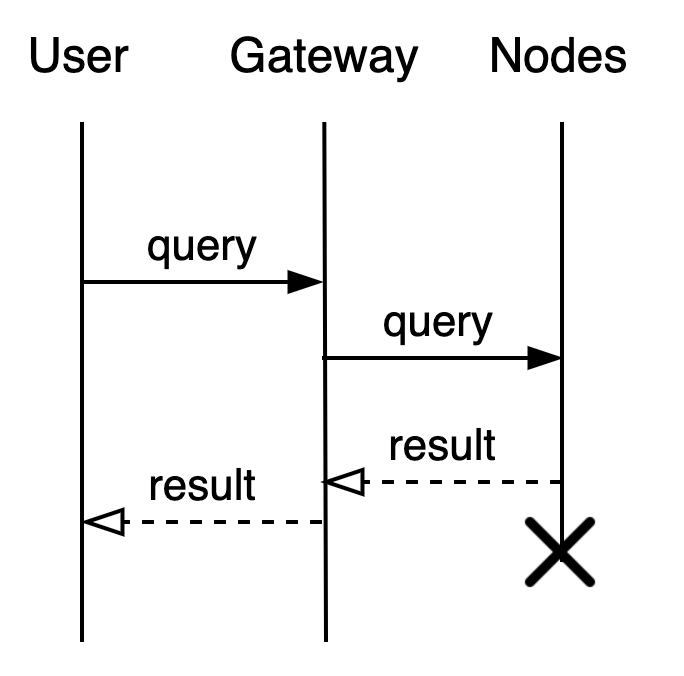
\includegraphics[scale=0.8]{images/Figure14}
	\end{center}
	\vspace{-0.7cm}
	\caption{Low level communication protocol diagram of query operation.}
	\label{fig:fig14}
\end{figure}
%
%
\subsection{Mutate}\label{sec:mutate} 
Mutate operation (orange arrows in Figure~\ref{fig:fig11}.) change the system state by creating, editing, or deleting clusters, regions, and topologies. When a user wants to perform a mutation over the system, a desired state needs to be specified \textbf{declaratively} using a YAML file, and submitted to the system. When state is submitted, the system will do the rest of the job to ensure that user desired state is reached.

The users specify which nodes are forming the cluster. Optionally, users can also specify labels and names on the node level, and retention period on the cluster level. The retention period is used to describe how long metrics are going to be kept. When the retention period expires, the metrics data will be deleted or moved to another location. 

Users can target a specific system queue, by adding a metadata part in the configuration file. With this ability, users can aim for specific queues just for the mutation to avoid long waiting times if other queues are full. Currently, the system do not have any limitations, restrictions or logic that will specify which queues are used for what or give them special rules or permissions. This can be views as a \say{gentleman agreement}, that in one team, operations users can proclaim specific queues like \textit{mutatation} queus used maybe for specific topologies, and latter on for other operarations as well.

When forming a topology, users can assign a name and labels to the entire topology. These parameters will be used when the user wants to query all topologies to get full information about regions, clusters, and nodes inside a topology

Mutate operation is \textbf{immutable} which mean that there will be no in place changes to the existing state. If user want to do any update, he needs to specify full new state that will replace existing state. This operation is \textbf{atomic} as well, which mean that whole new state must be able to replace existing state. Iff this happend, system will replace old state with the new state. Main storage that stores configuration data is key-value store implemented using etcd databse. Key that will be used to store the confuguration data is the whole path of topology, regions, cluster, node, while the value is user desired state. Listing~\ref{lst:listing4} show structure for key-value pair that is stored in main database, where on top we can see a structure of the \textbf{key}, and below it we can see structure of the \textbf{value}. This kind of structure is similar to OS file-system data organizations of files and folders.

\lstinputlisting[caption={Structure of stored key-value element.}, label={lst:listing4}, captionpos=b, xleftmargin=.25\textwidth]{listings/listing4.txt}

We store as well one additional information about labels \textbf{index} value. This index is used for faster querry of elements, when doing labels comparison. To find elements we can query on similar way like doing search in files and folders structure. The etcd in newer version \textbf{do not allow} hierarchical keyspace, but what they allow is \textbf{ranged} query by some \textbf{prefix}. This is useafull as well, because we can still get all regions in topology, clusters in region or nodes in the cluster if we know to which group they belog.

Mutate operaption is not idempotent by the nature, but whole process behind it make mutate an idempotent operation. Whether user try to create already existing infrastructure by changeing order of regions clusters or labes in the nodes, or if he for whatever reason did not get confirmation that infgrastructure is created a existing infrastructure will not be created. This is done in such a way, that $State$ service (Figure~\ref{fig:fig11}) will keep information set about created infrastructure. 

This informations is implemented as a \textbf{flat keyspace} set, that have information. On every mutation request, system will tets if such topology already exists. If such topology already exists user will get confirmation that his infrastructure is created. If such topology do not exists, a new cluster formation protocol~\ref{sec:cluster_formation_protocol} will be initiated.

The mutation confirmation is followed by unique id which user can use to query steps, logs and traces that are done in process of working towards user desired state. Logs service can give user comlete details about his task state using that unique id.

When creationg topologies, user is free to give whatever name he wants for every region, cluster and node. The only restrictino is that name should be alphanumeric set of characters.

Listing~\ref{lst:listing2} show example of user defined state that forms topology of one region with one cluster that contains three nodes, with retention period of 24h. Whole topology will have same set of labels, but $node3$ redefine this rule by specifying his own.

\lstinputlisting[caption=Example of mutate file using YAML., label={lst:listing2}, captionpos=b, xleftmargin=.3\textwidth]{listings/listing2.yaml}

After all nodes that should form a cluster, acknowledge cluster formation message, they will inform the system that the message is received, and they will start the process of cluster formation. This process is done by using SWIM~\cite{DasGM02}, a Gossip style protocol. When every node have complete list of his peers that should be in the cluster, the process of cluster formation is done. 

On the next health-check message, every node will send his \textbf{id} that is telling the sytem that he is part of some cluster. This kind of messages, will be used in $State$ service to validate that cluster is alive and well, or that some nodes (or all), are dead or down if \textbf{id} is not received. 

And Gossip style protocols (like SWIM) could be used in the future to propagate information in the cluster, without explicitly ping every node in the cluster.
%
%
\subsection{List}\label{sec:list}  
List command show the current state of the system for the logged user (blue arrows in Figure~\ref{fig:fig11}.). Logged user is able \textbf{only} to see infrastructure he created or he is maintaing. All other infrastructures, craeted by other users will not be visible to the users that are not creators or maintainers.

To view his infrastructures, the user can specify what part of the system he wants to see using set of labels or list of key-value pairs which will be used by the system to determine what user want to se. This process is similat to \textbf{selector} shown in the query~\ref{sec:query} operation. 

There are two levels of details that user can specify:

\begin{enumerate}[start=1,label={(\bfseries \arabic*)}]
	\item \textbf{global view}  of the syste, or all topologies he manages with just basic informations like resoource utilization, number of regions clusters and nodes.
	\item \textbf{detail view}, or details about a single topology (i.e., regions, clusters, and nodes in a single topology). Users can specify a more detailed view of a single cluster, meaning the users will get information about what resources the cluster has, but also resource utilization over time (using stored metrics information) and so on.
\end{enumerate}

Both options can be usefull if operations people need different details level for different topologies. 
%
%
\subsection{Logs}\label{sec:logs}
% 
The logs operation showing stored logs and traces to the user (purple arrows in Figure~\ref{fig:fig11}.). Same as previous operations, user needs to be registered and logged in to be able to performe this action. With this action, the user can see the state of his operations and actions. The user can choose between two options to querying his logs:

\begin{enumerate}[start=1,label={(\bfseries \arabic*)}]
	\item \textbf{get}, for this option user need to provide unique task id that is given to the uers when he creates a mutate operation. With this option user will get a full list of steps, traces and logs collected over the time the system was setting up his desired state.  
	\item \textbf{list}, with this option user can specify \textbf{selector} using list of key-value pairs in a similar way to query~\ref{sec:query} and mutate~\ref{sec:mutate} to filter only parts of the traces that contains same labels as selector does.
\end{enumerate}

This action is implemented in some basic aspects, as this action can return huge amoount of data that require some better visualizaion than CLI.
%
%
\section{Results}\label{sec:results} 
Framework described in previous section is put the the test. For ease of testing, we have used few ARM based nodes that easy to move from place to place. Test should be conducted on the heterogenious nodes, to see how the system will react on different architectures and resources. In our tests, we have used:

\begin{itemize}
	\item 9 Raspberry Pi 3+ Model B with 1GB LPDDR2 SDRAM, 16GB SDCard storage, and 1.4GHz Cortex-A53 64-bit SoC running Raspbian Linux, a Debian-based operating system.
	\item 3 Beagle bone black devices with 512MB DDR3 RAM, 4GB 8-bit eMMC on-board flash storage, and 1GHz ARM Cortex-A8 running a version of Linux Debian operating system.
\end{itemize}

\noindent
as test heterogenious nodes for creating clusters, regions, and topologies. 

Using Go tooling, we were able to build daemon service without changes and dissiminate on all nodes without problems.

We have run tests on different configurations and different nodes clusters using these nodes. All nodes were connected on the network, and experiments were conducted in a controlled environment. Nodes that should be part of the same claster are connected on same network for easier experiments.

Experimental research was realized in the laboratory of the Department of Informatics at the Faculty of Technical Sciences in Novi Sad. The laboratory of the Department of Informatics is equipped with adequate computer, communication and software equipment on which the set goals in this thesis can be fully realized.
%
%
\section{Applications}\label{sec:app}
%
This research focus on a platform with geo-distributed edge nodes can be organized dynamically into the micro data-centers and regions based on the cloud model, but adapted for a different environment. This middle layer helps the power-hungry servers reduce traffic by serving the nearby population requests and possibly syncing their data without expensive consensus protocols~\cite{inproceedingsSimic2}. These micro data-centers or micro clouds also increase the availability and reliability of the cloud services, and as such could be offered as a service to users.

With clear separation of concerns and a familiar application model for the users it opens possibilities for new human-centered applications, for example, area traffic control. 

If we imagine a scenario where a new catastrophic event (earthquake, tsunami, war, terrorist attack, pandemic, etc.) is in the human population, an increasing amount of ambulance vehicles must be routed to hospitals fast, in the city area for example. The traffic control system suddenly needs more resources to continue operating properly. On top of that, if the healthcare system is like the one presented in~\cite{OmarBBKR19, inproceedingsSimic5}, we can monitor patient health in real-time~\cite{Al-KhafajiyBCAK19} and transfer data to the healthcare platform. 

This gives health workers crucial information about patients on their arrival. Resource vise, this scenario is relatively easy to solve if using the cloud, as we increase resource demand. The main advance of EC, when compared to the cloud only approach, is the acceleration of the communication speed. In our scenario, the cloud could bring huge latency, while EC originates from peer to peer systems~\cite{LopezMEDHIBFR15}, serving only local population needs, minimizing potentially huge round-trip time of the cloud. Furthermore, our model expands peer to peer systems into new directions and blends them with the cloud to allow novel human-centered, cloud-like applications. 

For applications like self-driving cars, delivery drones, or power balancing in electric grids require real-time processing for proper decision making, or any other application that future developers may develop.

Users are getting a new platform as a blank canvas, and there is no limitation in what applications they can develop. Integrating hardware and/or software even more, connecting sensors and things around us and eventually an operating system that will be capable of running city/state infrastructure without human intervention.
%
%